\section{Práctica de laboratorio}

La práctica de laboratorio consistió en medir analizar el comportamiento de un termistor como sensor de temperatura, cuyo coeficiente de temperatura es negativo. 
Para ello, se realizaron dos pruebas por separado: la medición del valor resistivo con un multímetro y con un programa de Arduino.
\subsection{Medición con multímetro}
Por un lado, se empleó el dispositivo en su función de medición de resistencias u óhmetro para registrar el valor resistivo del termistor bajo
tres condiciones: a temperatura ambiente, a altas temperaturas y bajas temperaturas. Para ello se procedió de la siguiente manera:
\begin{enumerate}
    \item Se conectó el termopar a las conexiones del multímetro que permiten esta función. Para el caso de temperatura ambiente, se sostuvo el elemento en la mano, resguardado del aire acondicionado; para la temperatura alta, se colocó en un vaso
    descartable con agua caliente tomada del dispenser y, para las temperaturas bajas, se introdujo en otro vaso descartable con hielo.
    \item En cada caso, se enroscaron los conectores metálicos del termistor a las puntas del multímetro, en función de óhmetro, y se registró su valor de resistencia en $ \omega$.
    \item Se tabularon tanto la temperatura en °C y la resistencia para realizar la segunda parte del trabajo.
\end{enumerate}

\subsection{Medición con arduino}
Seguidamente, se empleó el circuito presentado en la figura con un Arduino UNO. Éste es un microprocesador de 20 pines y alimentado con 5 V mediante una batería externa, al cual se le carga un programa en lenguaje C mediante el software \textit{IDE Arduino} con instrucciones a realizar según
sus conexiones. Adicionalmente, este microprocesador cuenta con conversores analógico- digitales (ADC) internos, los cuales permiten levantar señales del primer tipo y convertirlas al segundo para poder ser leídas y procesadas en otros dipositivos. 
Particularmente en este caso, se construyó el circuito con el termistor y una resistencia, conectados a un pin de alimentación y a otro del ADC para poder leer tanto el valor resistivo del termistor como la temperatura a la cual se encuentra. Esto fue posible gracias al código compartido por la cátedra,
el cual tenía ingresada la ecuación de Steinhart - Hart, que establece una relación entre la resistencia eléctrica de un semiconductor y la temperatura a la que está sometido. Primero, se realizaron las mismas tres mediciones anteriores empleando los coeficientes del fabricante y se tabularon los registros.
\begin{figure}[H]
    \centering
    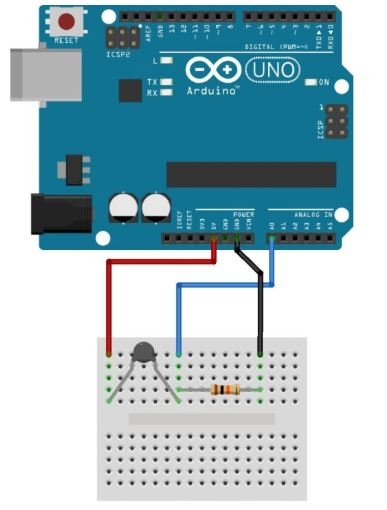
\includegraphics[width=0.4\textwidth]{figuras/Esquema circuito.JPG}
    \caption{Esquema del circuito empleado}
    \label{fig:mi_imagen}
\end{figure}

En una segunda instancia, empleando los valores de las mediciones con el multímetro, se procedió a calcular los coeficientes del termistor que obedecen a la ecuación de Steinhart - Hart, utilizando la página web \textit{Steinhart - Hart equation calculator} \footnote{Link de acceso: https://rusefi.com/Steinhart-Hart.html}, la cual tiene tres pares de entradas: resistencia y temperatura para los casos caliente, frio y ambiente.
En ella se ingresaron dichos valores y se obtuvieron los coeficientes correspondientes. Se realizaron las mismas tres mediciones nuevamente, y se analizó comparativamente con los resultados alcanzados con los coeificentes del fabricante.


